%--------------------------------------------------------------------------------------
% Dokumentum formátuma [Document format]
%--------------------------------------------------------------------------------------
\documentclass[12pt,a4paper,oneside]{article}

%--------------------------------------------------------------------------------------
% Csomagok inicializálása [Initializing packages]
%--------------------------------------------------------------------------------------

\usepackage[utf8]{inputenc}
\usepackage[magyar]{babel}
\usepackage{t1enc}
\usepackage{amsmath}
\usepackage{amsfonts}
\usepackage{amssymb}
\usepackage{geometry}
\geometry{
    top=20mm,
    bottom=20mm,
    left=20mm,
    right=20mm,
}
\usepackage{hyperref}
\usepackage{mathrsfs}
\usepackage{fancyhdr}
\usepackage{graphicx}
\usepackage{icomma}
\usepackage{adjustbox}
\usepackage{lastpage}
\usepackage{float}
\usepackage{pdfpages}
\usepackage{subcaption}
\usepackage{tocloft}
\usepackage{bm}
\usepackage{multicol}
\usepackage{listings}
\usepackage{tikz}
\usepackage[abs]{overpic}
\usepackage{pict2e}

%--------------------------------------------------------------------------------------
% Dokumentum törzse [Document body]
%--------------------------------------------------------------------------------------

\begin{document}

%--------------------------------------------------------------------------------------
% Címoldal [Titlepage]
%--------------------------------------------------------------------------------------

\author{\textit{Készítették:}\\ Buczny Dominik \hspace{5pt} Hanich Péter \\ Németh Gergő Olivér \hspace{5pt} Olchváry Ambrus \\[10pt] \textit{Konzulens:}\\ Gazdi László}
\title{Szoftverarchitektúrák Házi Feladat \\ Író-olvasó oldal \\ \textbf{Specifikáció}}
\date{2024/2025/1}
\maketitle
\thispagestyle{empty}
\begin{center}
    
\includegraphics[width=\textwidth,height=\textheight,keepaspectratio]{./figures/logo.png}
\end{center}  

%--------------------------------------------------------------------------------------
% Tartalomjegyzék [Table of Contents]
%--------------------------------------------------------------------------------------
\newpage
\tableofcontents
\thispagestyle{empty}
\newpage

%--------------------------------------------------------------------------------------
% Oldalszámok formázása [Page numbering]
%--------------------------------------------------------------------------------------
\fancyhf{}
\lhead{Szoftverarchitektúrák}
\rhead{VIAUMA21}
\cfoot{\thepage}
\pagestyle{fancy}
\setcounter{page}{1}


%--------------------------------------------------------------------------------------
% Tartalom [Contents]
%--------------------------------------------------------------------------------------

%TODO A tartalmat ide írd  [Write the chapters here]
% Ki lehet file-okba is szervezni [You can organize it into files]
% Példa: \include{sections/introduction}

\section{A rendszer célja, funkciói, környezete.}

\subsection{Feladatkiírás}
A feladat egy író-olvasó oldal elkészítése. Az oldalon a regisztrált felhasználók olvashatják egymás megosztott történeteit, azokhoz megjegyzéseket, kritikákat fűzhetnek. A történeteket legyen lehetőség gyűjteményekbe, a fejezeteket regényekbe szervezni. A feltöltött történetek minden esetben moderátori ellenőrzésen esnek át, csak ez után érhetőek el publikusan. A moderálás eredményéről a felhasználót mindenképpen értesíteni kell. A történeteket el lehet látni jellemzőkkel, illetve meg lehet jelölni a kategóriájukat, a benne szereplő karaktereket, valamint figyelmeztetéseket és korhatárt lehet rájuk beállítani. Ezen kívül a regisztrált felhasználóknak lehetőségük van egymással privát üzenetben kommunikálni. A rendszerhez webes és mobilos kliens készítése is szükséges.
A részletes követelmények a \textit{Specifikáció} dokumentumban találhatók.
Mi a feladatkiírástól némileg eltérő nevezéktant használtunk: a továbbiekban a \textit{történet} helyett a \textit{mű} szót használjuk.

\subsection{A rendszer által biztosított funkciók}

A specifikáció alapján a platform a következő főbb funkciókat hivatott biztosítani. 
(Az egyes funkciók különböző szintű jogosultságokhoz kötöttek lehetnek.):
\begin{itemize}
    \item  Regisztráció
    \item  Bejelentkezés
    \item  Művekkel kapcsolatos funkciók:
    \begin{itemize}
        \item Történetek böngészése
        \item Történetek keresése
        \item Történetek olvasása
        \item Történetek létrehozása
        \item Történetek szerkesztése, fejezetekre osztása
        \item Történetek moderálása

    \end{itemize}
    \item  Gyűjteményekkel kapcsolatos funkciók:
    \begin{itemize}
        \item Gyűjtemények böngészése
        \item Gyűjtemények keresése
        \item Gyűjtemények megtekintése
        \item Gyűjtemények létrehozása 
    \end{itemize}
    \item  Hozzászólás írása Művekhez vgy Gyűjteményekhez
    \item  Művek, Gyűjtemények, Hozzászólások kedvelése
    \item  Privát üzenetek küldése
\end{itemize}

A rendszer az alábbi szerepköröket különbözteti meg: látogató, regisztrált felhasználó, moderátor, adminisztrátor. 
A látogatók csak a megosztott tartalmakat tekinthetik meg, a regisztrált felhasználók létrehozhatnak saját tartalmat, kommentelhetnek, kedvelhetnek és üzeneteket küldhetnek.
A moderátorok a moderálási jogosultságokkal rendelkeznek, az adminisztrátorok pedig a teljes rendszer felett rendelkeznek, kezelik a jogosultságokat.

\subsection{A rendszer környezete}

--- Backend és web környezetének leírása ---

A mobil kliens platformspecifikus, android operációs rendszerre készült kotlin nyelven Android Studioban.
A felhasználói felület normál méretű mobiltelefonra lett optimalizálva, egyéb méretű eszközökön (pl. okosórán) nem lett tesztelve.
A mobil kliens használatához internetelérés szükséges, az alkalmazás elérje  a backend szolgáltatásokat. 

\section{Megvalósítás}
\label{sec:implementation}


A szoftver három fő komponensből áll össze: a backend, a webes kliens és a mobil kliens.
A hárokomponens klasszikus kliens-szerver architektúrát valósít meg: a backend a szerveroldali logikát, a webes és a mobilos kliens 
felhasználói felületet.
A backend és a kliensek közötti kommunikáció http protokollon keresztül történik, a backend REST API-t biztosít a kliensek számára.
Az egyes komponensek fejlesztését, külön külön végeztük, így a fejlesztőcsapat tagjainak jól elkülönülő feladata és felelősségi körük volt.
\subsection{Architektúra}

A szoftver egészében és komponenseiben is rétzegzett architektúrát valósít meg, melynek egy áttekintő ábrája látható a \ref{fig:architecture} ábrán.

\begin{figure}[H]
    \centering
    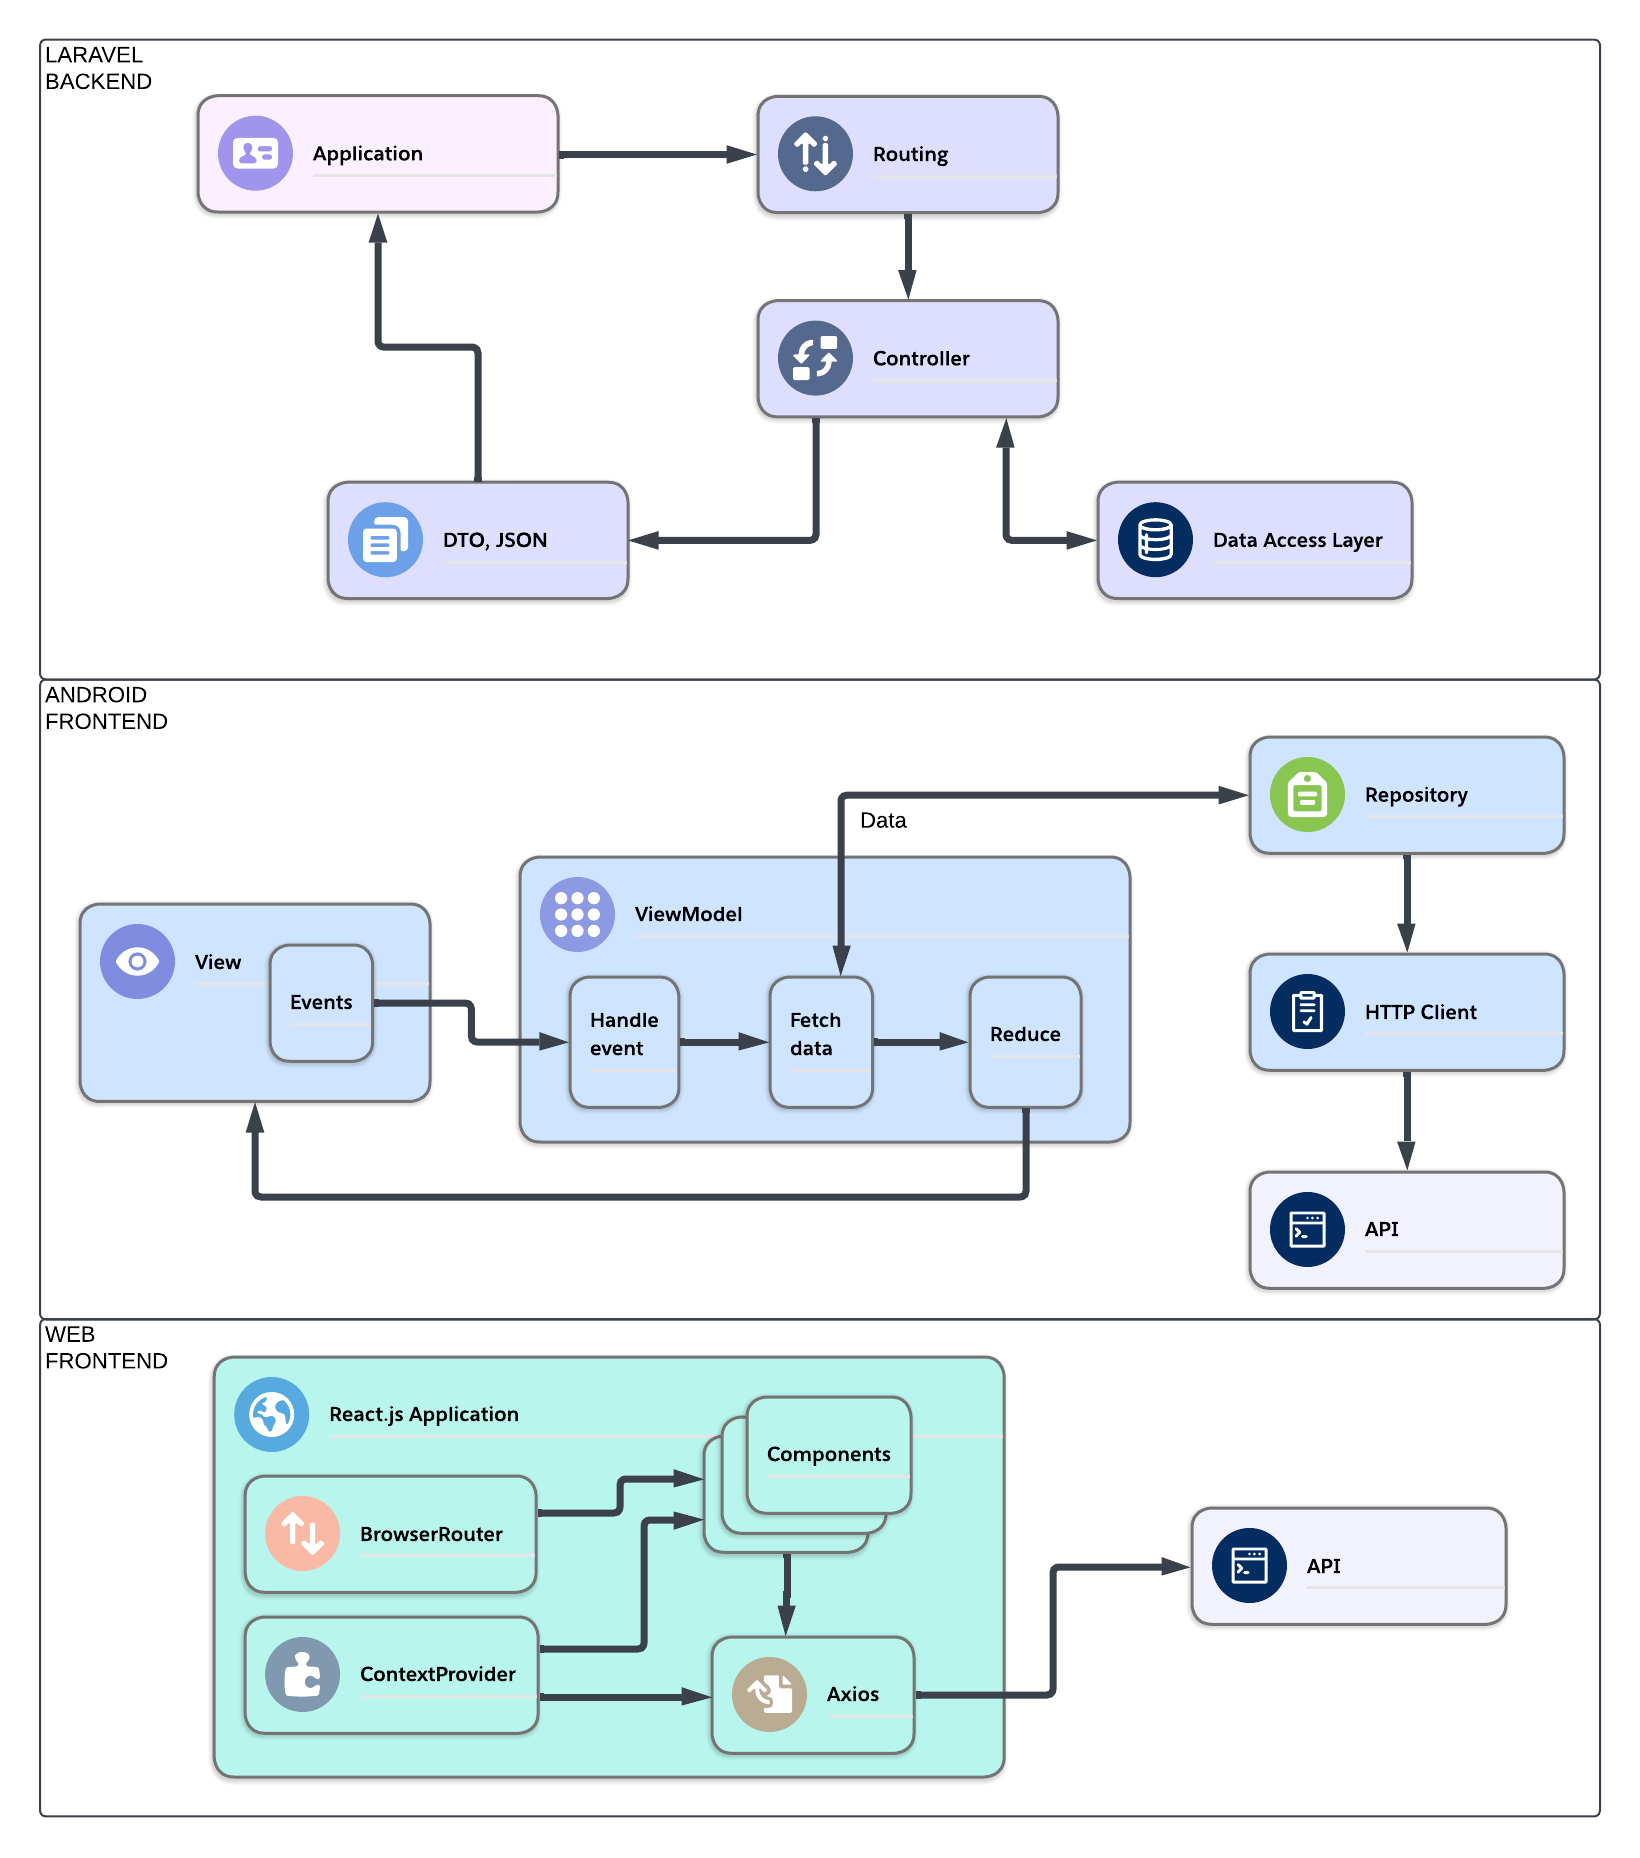
\includegraphics[scale=0.5]{./figures/architecture.png}
    \caption{A szoftver architektúrája}
    \label{fig:architecture}
\end{figure}

A szoftver egy kliens-szerver architektúrát valósít meg, ahol a kliensek a szerverrel REST API-n keresztül kommunikálnak. A szerver oldali alkalmazás a Laravel PHP keretrendszer segítségével készült, míg a kliens oldali alkalmazás két részre osztható: egy webes frontendre, mely a React keretrendszerre épül, és egy mobil kliensre, mely a JetPack Compose keretrendszer segítségével készült.

\subsubsection{Backend architektúra}

A Laravel alapból az MVC (Model-View-Controller) architektúrát követi, azonban a projektünkben a nézeteket a kliensek kezelik, így csak a Modell és a Controller rétegek maradnak meg. Így a Laravel alkalmazásunk 2 fő rétegre osztható:

\begin{itemize}
    \item Adathozzáférési réteg (Data Access Layer)
    \item Üzleti logikai réteg (Business Logic Layer)
\end{itemize}

A kliensekkel való kommunikáció REST API-n keresztül történik, így a Laravel alkalmazásunkban a REST API végpontok implementációja a kontrollerekben található. A küldött és fogadott adatok JSON formátumban vannak, melyek a Laravel által biztosított Resource osztályok segítségével könnyen kezelhetőek, melyek egyfajta DTO (Data Transfer Object) mintaként működnek.

\subsubsection{Mobilos kliens}

A mobilos kliens 2 fő rétegre osztható:

\begin{itemize}
    \item  [1.] Adat réteg (Data Layer)
    \begin{itemize}
        \item Adatlekérdezési réteg (HTTP kliens): REST API hívások implementációja, JSON objektumok kotlin osztályokra való leképezése.
        \item Adatelérési réteg (Repository): hálózati kommunikáció és hibakezelés és egységesített kezelése, magasabb szintű kódban könnyebben használható.
    \end{itemize}
    \item  [2.] UI réteg (UI Layer)
    \begin{itemize}
        \item  Állapotkezelés (View Model)
        \item  Megjelenítés (View)

    \end{itemize}
\end{itemize}

\subsubsection{Webes frontend}

A webes kliens REACT-ot használ és ebből adódóan egy SPA (Single-Page Application), amely komponensekkel építi fel a virtuális DOM-t, állapotok és események vezérlik.


%--------------------------------------------------------------------------------------
% Bibliográfia [Bibliography] - Ha üres kommenteld ki [Uncomment if empty]
%--------------------------------------------------------------------------------------

%\newpage
%\thispagestyle{empty}
%\pagenumbering{gobble}
%{
%    \footnotesize  % Kisebb betűméret [Smaller font size]
%    \bibliographystyle{plain}
%    \bibliography{mybib}
%}
%\addcontentsline{toc}{section}{Hivatkozások}

\end{document}